\chapter{L'inflation}
\newthought{L'inflation}\index{inflation} désigne une phase de l'histoire de l'Univers durant laquelle l'espace aurait rapidement 'enflé', avec des taux d'expansion exponentiels. Cet épisode aurait pris place environ $10^{-34}$ secondes après le Big-Bang\index{Big-Bang} et a été suggéré à partir des années 1980 pour expliquer toute une série de défis qui se posent quant à l'état de l'Univers tel que nous l'observons. L'époque inflationnaire reste pour l'instant une hypothèse non vérifiée expérimentalement mais pour laquelle existe tout un faisceau de présomptions.

\section{Pourquoi l'inflation ?}
\subsection{Le problème de l'Horizon de causalité}
\newthought{Le principe cosmologique}\index{principe cosmologique} repose sur une hypothèse d'homogénéité\index{inflation!homogénéité} de l'Univers et cette homogénéité n'est pas remise en question aujourd'hui par les observations. L'une des manifestations les plus spectaculaire de cette homogénéité est la température du fond diffus cosmologique~: comme expliqué dans le chapitre dédié, le fond diffus cosmologique présente une température typique $T\sim 2.7 $K à un très haut niveau de précision (à $10^{-5}$ près) et ceci quelle que soit la direction vers laquelle on regarde \sidenote{on rappelle que c'est cette isotropie qui intrigua Penzias \& Wilson lors de leur découverte du signal}. 

Des anisotropies existent mais elles sont noyées dans l'amplitude du signal du monopole~ : on peut citer l'empreinte des oscillations baryoniques accoustiques\index{BAO}, déclenchées par la compétition entre gravité et pression de rayonnement, qui produisent ces grands pics dans le spectre de puissance angulaire du fond diffus. En particulier, les plus grandes échelles angulaires associées à ces ondes accoustiques sont de l'ordre du degré sur le ciel \sidenote{correspondant à une fréquence angulaire $\ell\sim 1000$}. Cette échelle angulaire correspond à \textit{l'horizon sonore} \index{horizon}aux époques de l'émission du fond diffus~: cet horizon est la plus grande distance qui peut être parcourue à la vitesse du son dans les conditions qui régnaient dans l'Univers à ces époques. Cette vitesse du son est régie par la pression du rayonnement et est de l'ordre de :
\begin{equation}
c_s\sim \frac{c}{\sqrt 3}.
\end{equation}
tandis que l'horizon peut-être approximé par:
\begin{equation}
L_H\sim\frac{c_s}{H}
\end{equation}
On constate donc aisément que l'horizon sonore est proche de l'horizon causal, déterminé lui par la vitesse de la lumière.

Nous avons donc une surface de dernière diffusion qui est isotrope à un très haut niveau de précision \textit{sur toute la sphère céleste} tandis que les échelles de longueurs en contact causal (donc de taille inférieure à l'horizon) sont particulièrement ramassées. Par conséquent, on ne peut trouver de processus physiques qui soit en mesure de propager une information sur tout le ciel 380 000 ans après le Big-Bang : cette homogénéité et isotropie ne peut trouver son origine dans un mécanisme physique qui aurait établi ces propriétés sur ces très grandes échelles sans lien causal.

\newthought{Deux possibilités} s'offrent à nouveau : cette isotropie est une condition initiale, particulière mais établie sans raison aucune ou bien cette isotropie est bien le fruit de la propagation d'un signal physique mais sur des échelles plus faibles que celles sur lesquelles l'isotropie est aujourd'hui observée. L'inflation intervient dans ce second scénario : une théorie de l'inflation stipule que l'on ne peut extrapoler l'histoire d'expansion de l'Univers vers le Big-Bang à partir de son contenu actuel et donc de sa dynamique actuelle. Il faut invoquer un épisode où le paramètre d'expansion $a(t)$ connaît une variation soudaine, faisant traverser l'horizon à des échelles en initialement en lien causal. L'idée est simple~: les plus grandes échelles observées sur le ciel étaient sous l'horizon avant l'épisode inflationnaire et sont passées hors-horizon après ce dernier. 

La figure \ref{inflation} illustre les possibilités ouvertes par une période d'inflation. Pendant les périodes d'expansion 'normales', la taille physique de l'horizon est donnée par :
\begin{equation}
L_H=\frac{c}{H}=a^p
\end{equation}
avec $p=2$ durant l'époque de domination du rayonnement puis $p=3/2$ durant l'époque de domination de la matière. De même une distance donnée évolue sous l'effet de l'expansion exactement comme le facteur d'expansion, $L\sim a$. Par conséquent, au cours du temps, un mode de taille comobile donnée va d'abord être plus grand que l'horizon puis plus petit que l'horizon : un mode plus grand que l'horizon à un instant donné l'était forcément dans le passé, des régions sans lien causal dans le CMB ne l'ont jamais été auparavant. 

\begin{figure}[htbp]
	\centering
		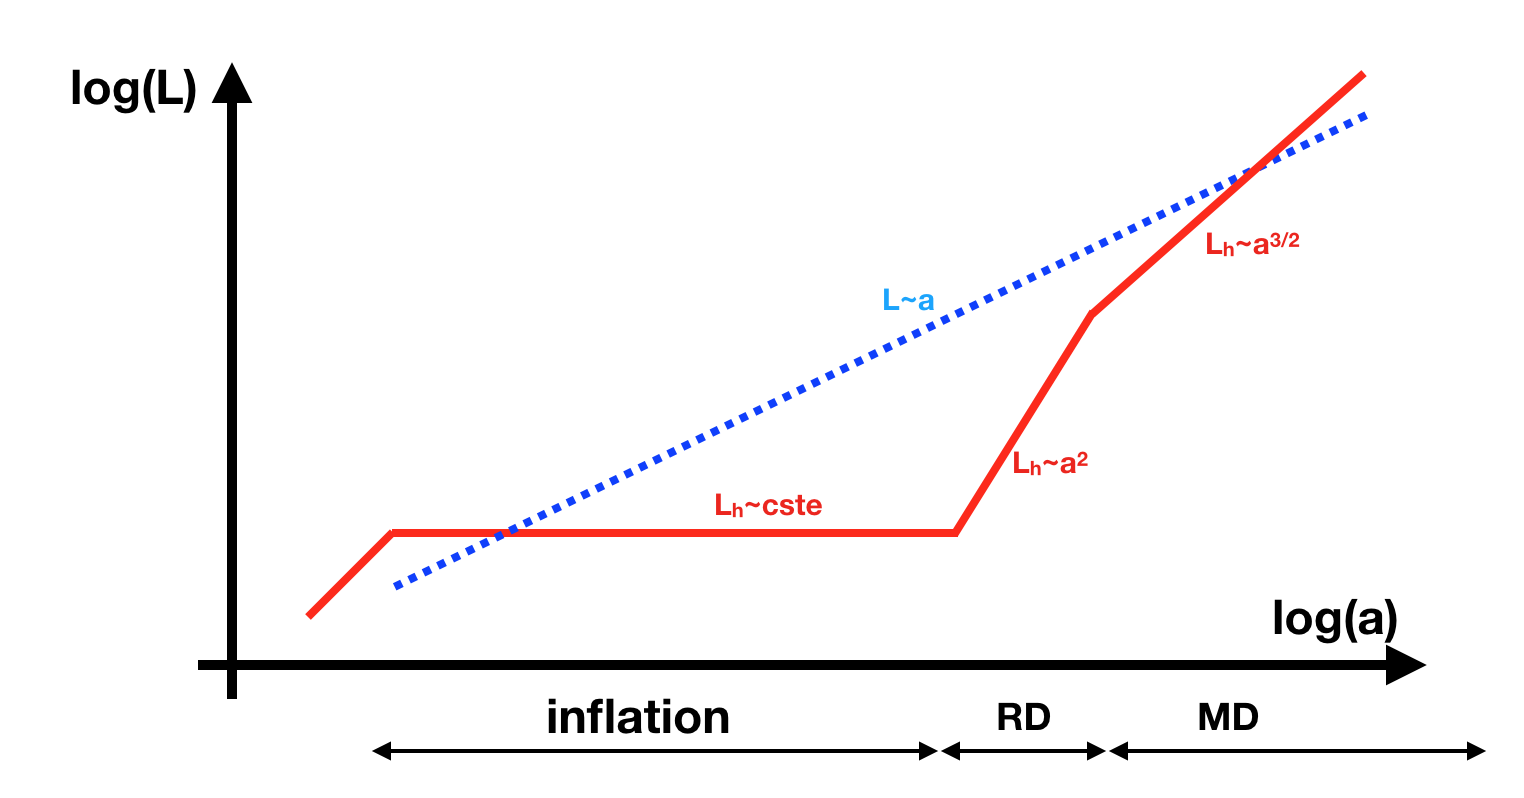
\includegraphics[height=25cm]{figs/inflation.png}
	\caption[Histoire d'évolution de quelques longeurs physiques au cours du temps.]{Histoire d'évolution de quelques longeurs physiques au cours du temps. $L_H$ désigne l'horizon, dont la taille physique est constante durant l'inflation, tandis que $L$ désigne la taille physique d'un mode de taille comobile donnée.$RD$ et $MD$ désigne les périodes de domination du rayonnement et de la matière, respectivement. }
	\label{f:inflation}
\end{figure}

Compte tenu des échelles en jeu\sidenote{on rappelle que l'isotropie est observée sur toute la surface de dernière diffusion, dont le rayon est de l'ordre de plusieurs Gpc}, cette inflation doit impliquer des croissances gigantesques. On verra par la suite que les distances doivent s'accroître typiquement d'un facteur $10^{30}$.


\subsection{Le problème de la platitude}
\newthought{La géométrie de l'Univers est plane} en moyenne et sur des distances cosmologiques. Dans une telle géométrie, la lumière se propage en ligne droite et la somme des angles d'un triangle fait 180 degrés : comme expliqué dans le chapitre dédié, la taille angulaire des oscillations baryoniques accoustiques mesurée dans le fond diffus à $z\sim1100$ ou dans les grands relevés de galaxies à $z\sim 0$ est hautement compatible avec ce type de géométrie. Un Univers sphérique a tendance à surestimer ces tailles angulaires, un Univers hyperbolique à les sous-estimer et de fait la réalité terrain semble indiquer que le régime à l'oeuvre est exactement entre ces deux situations.

Tout comme le problème de la causalité, le fait d'avoir une géométrie plane\index{inflation!géométrie plane} peut soit être le fruit d'un mécanisme qui aurait aplati une géométrie arbitraire ou bien la conséquence d'un choix de conditions initiales particulier. Et à nouveau cette seconde option n'est pas entièrement satisfaisante: en effet le départ à la platitude peut s'exprimer via l'équation suivante:
\begin{equation}
|1-\Omega|=\frac{k}{a^2 H^2}\sim t
\end{equation}
où la dernière approximation suppose un Univers dominé par le rayonnement comme c'est le cas dans un Univers très jeune \sidenote{on rappelle que dans ce régime $a(t)\sim \sqrt{t}$}. On constate aisément que $1-\Omega$ tend à s'écarter de zéro avec le temps, donc si l'Univers possède une géométrie plane aujourd'hui, sa platitude devait être encore plus affirmée dans le passé~: en supposant par exemple que $\Omega$ est de l'ordre de l'unité à l'unité près aujourd'hui alors:
\begin{equation}
\Omega (t=13.8 \mathrm{Gyrs}) \sim \mathcal{O} (1) \rightarrow |1-\Omega (t=180 \mathrm{sec})| \sim \mathcal{O} (10^{-16}).
\end{equation}
où 180 secondes correspond à la nucléosynthèse primordiale et le problème va en s'accentuant si l'on s'approche du Big-Bang.
Dès lors, il est difficile d'imaginer un tirage aléatoire de ce paramètre qui soit si proche de l'unité dans ces instants reculés. En proposant une augmentation exponentielle des distances, l'inflation fournit naturellement \textit{un mécanisme} pour gommer toute sorte de courbure~: l'Univers était peut-être doté d'une courbure non-nulle à une époque reculée mais l'Inflation aurait fait tendre toute courbure initiale non nulle vers zéro. Tout rayon de courbure raisonnablement non nul verrait sa valeur augmenter d'un facteur $10^{30}$, donnant l'apparence d'une géométrie plane.

\subsection{L'origine des fluctuations cosmiques}
\newthought{Les grandes structures de l'Univers} trouvent leur origine dans l'existence de fluctuations\index{inflation!fluctuations} dans la distribution spatiale de la densité d'énergie (ou de matière). Ces fluctuations sont observées à de très faibles niveaux dans le fond diffus cosmologique et ce sont ces 'graines' qui servent de point d'ancrage au processus d'instabilité gravitationnelle. Sans ces fluctuations, pas de structures dans l'Univers actuel. 

Comme indiqué précédemment, on attend d'une période inflationnaire qu'elle conduise à un accroissement des échelles de longueurs d'un facteur $\sim 10^{30}$. Si l'on prend une structure de taille 10 Mpc aujourd'hui, un tel facteur conduit à  une taille initiale de l'ordre de $10^{-8}$ m, c'est à dire des échelles soumises à des processus quantiques. Par conséquent, on peut imaginer que les structures observées aujourd'hui sont le fruit du passage à l'échelle macroscopique de fluctuations quantiques, par le biais de l'Inflation. 

De façon générique, ces fluctuations quantiques sont invariantes d'échelles: il n'existe pas de taille caractéristique dont on attend qu'elle domine 'le bruit' de fluctuations. Les spectre de puissance des fluctuations attendues ne doit pas présenter d'échelle particulière et l'une des prédictions générale des modèles d'inflation est la mise en place de fluctuation dont le spectre de puissance est une simple loi de puissance:
\begin{equation}
P_\mathrm{inflation}\sim k^n
\end{equation}
où $n$ est entier proche de l'unité.

\subsection{Les particules reliques}
\newthought{Un problème plus subtil} posé par le modèle d'expansion standard est l'absence aujourd'hui de certaines certaines particules dont la production est pourtant prédite dans un Univers dense et chaud. C'est le cas par exemple des \textit{monopôles} magnétiques\index{inflation!monopôle magnétique}\index{particules reliques}, qui seraient des analogues aux charges électriques \sidenote{ces monopôles magnétiques seraient en mesure de créer des champs magnétiques divergents ou convergents ($\vec \nabla \vec B \neq 0$). Aujourd'hui seuls les courants de charges électriques sont en mesure de générer un tel champ, configuré en 'boucles de champs magnétiques' ($\vec \nabla \vec B \neq 0$).}~: il n'existe pas à priori de raisons pour lesquelles ces particules sont indétectables dans notre Univers. En particulier, leur contribution au bilan énergétique de l'Univers doit, au pire, dominer celle du rayonnement\sidenote{la densité d'énergie des reliques décroît en $a^{-3}$ tandis que celle du rayonnement décroît en $a^{-4}$.}
On cite également souvent les axions ou bien les défauts topologiques, qui souffrent de la même absence aujourd'hui.
L'inflation fournit un mécanisme permettant de faire 'disparaître' ces objets: si ces objets sont produits avant une phase d'inflation rapide, alors cette phase va provoquer une dilution extraordinaire de leurs abondances. 

\section{Modèles d'inflation}
Cherchons à présent à développer un modèle plus quantitatif de l'inflation. Le point de départ naturel est lié au problème de la platitude de l'Univers : pour mémoire les densités d'énergies des différents fluides cosmiques sont liées par 
\begin{equation}
|1-(\Omega_m+\Omega_r+\Omega_v)|=|\Omega_k|=\frac{|k|}{a^2H^2}.
\end{equation}
où $k$ est lié à la courbure intrinsèque de l'Univers\index{courbure}. L'objectif de l'inflation est de faire tendre $\Omega_k$ vers zéro, pour aplatir la géométrie de l'Univers : idéalement cela peut s'obtenir en augmentant le facteur d'échelle $a$ de façon importante tout en empêchant $H(a)$ de diminuer. Il s'avère que nous avons déjà rencontré ce type de comportement, dans le cas d'un Univers dominé par l'énergie du vide à densité d'énergie constante et pour lequel nous avions une expansion accélérée avec $H(a)$ constant. Les modèles d'inflations vont invoquer le même type de comportement, à savoir:
\begin{eqnarray}
a&\sim&\exp{Ht}\\
H(a)&=&\mathrm{constante}.
\end{eqnarray} 
Par conséquent, les modèles d'inflations vont reposer sur une densité d'énergie constante, comme nous l'avions rencontré dans le cas de l'énergie du vide. La difficulté toutefois est le fait que l'inflation a une durée finie, circonscrite aux premiers instants de l'histoire de l'Univers~: il faut donc que le mécanisme garantisse aussi la disparition de cette densité d'énergie inflationnaire, pour que l'expansion puisse retrouver son comportement standard.

Ce type d'expansion permet de revisiter le problème de l'horizon\index{horizon} mentionné précédemment et illustré dans la figure \ref{f:inflation}. Durant la période d'inflation, l'horizon possède une taille physique constante :
\begin{equation}
L_H=\frac{c}{H}=\mathrm{constante}.
\end{equation}
Par conséquent, un mode de taille comobile donnée peut être successivement plus petit que l'horizon, puis plus grand au cours de l'inflation et éventuellement redevenir plus petit ultérieurement. Des régions sans lien causal au moment de leur observation ont ainsi pu être en contact causal antérieurement.


\subsection{L'inflaton}
\newthought{Les modèles standards d'inflation} repose sur la description d'un \textit{champ physique} appelé \textit{l'inflaton}\index{inflation!inflaton}. Un champ physique\index{champ physique} est défini en tout point de l'espace et du temps et peut sous certaines conditions être amené à se manifester sous formes de particules : c'est par exemple le cas du champ électromagnétique qui peut se manifester sous la forme de photons et de la même manière les électrons sont la manifestation d'un champ physique sous-jacent. Ces champs peuvent être scalaires, vectoriels voire tensoriels : cela défini notamment la façon dont leur perception est modifiée en fonction du système de référence utilisé.

Les modèles d'inflation reposent l'inflaton\index{inflation!inflaton} qui est généralement décrit sous la forme d'un champ scalaire, dont la valeur ne change pas sous l'effet d'un changement de système de référence et dans un Univers homogène, sa valeur ne peut dépendre de la position. Ce champ scalaire, qui remplit tout le cosmos, est noté $\phi(t)$. Ce champ, quantique, va créer les fluctuations d'énergie et de densité initiales et va imprimer des irrégularités, y compris sur un Univers parfaitement homogène à ses débuts. On peut également montrer que l'inflaton va imprimer des fluctuations tensorielles sur la métrique de l'espace-temps, qui se manifestent sous la forme d'ondes gravitationnelles primordiales.

Comment décrire l'évolution de ce champ ? La façon naturelle proposée par la théorie quantique des champs est d'associer à l'inflaton un potentiel qui dépend de sa valeur $V(\phi)$ \index{inflation!potentiel} ce potentiel associe une énergie à la valeur du champ et ce champ évolue dans ce potentiel comme dans une énergie potentielle\index{energie@énergie potentielle}. Par exemple, ce champ va dévaler les pentes de potentiels vers son minimum ou bien osciller dans des vallées de potentiels ou bien rester en équilibre sur les extrema de $V(\phi)$ \sidenote{de façon tout à fait analogue à la dynamique d'un système dans le champ énergie potentielle}. On peut également montrer que la densité d'énergie et la pression de l'inflaton sont données par \sidenote{on adopte ici le choix d'unité habituel de la théorie des champs qui permet d'écrire $c=\hbar=1$} 
\begin{eqnarray}
\rho_\phi&=&\frac{\dot \phi^2}{2}+V(\phi)\\
p_\phi&=&\frac{\dot \phi^2}{2}-V(\phi)\\
\end{eqnarray}
Ces expressions peuvent être réutilisées par exemple dans les équations de Friedmann pour calculer l'expansion associée à $\phi$. Par exemple on peut montrer que le paramètre de Hubble évolue selon:
\begin{equation}
H^2=\frac{8\pi G}{3}\left(\frac{\dot \phi^2}{2}-V(\phi)\right).
\label{e:hubbleinf}
\end{equation}
De même on peut éecrire l'équation de conservation de la densité d'énergie associée :
\begin{equation}
\dot \rho_\phi= -3H\rho_\phi-3Hp_\phi
\end{equation}
qui explicite simplement que la variation d'énergie au cours du temps est due à la dilution cosmologique (premier terme du membre de droite) et au travail des forces de pression (second terme du membre de droite). En terme d'inflaton, cette équation de conservation devient:
\begin{equation}
\ddot \phi+ 3H \dot \phi = -\frac{d V}{d\phi}
\end{equation}


\begin{figure}[htbp]
	\centering
		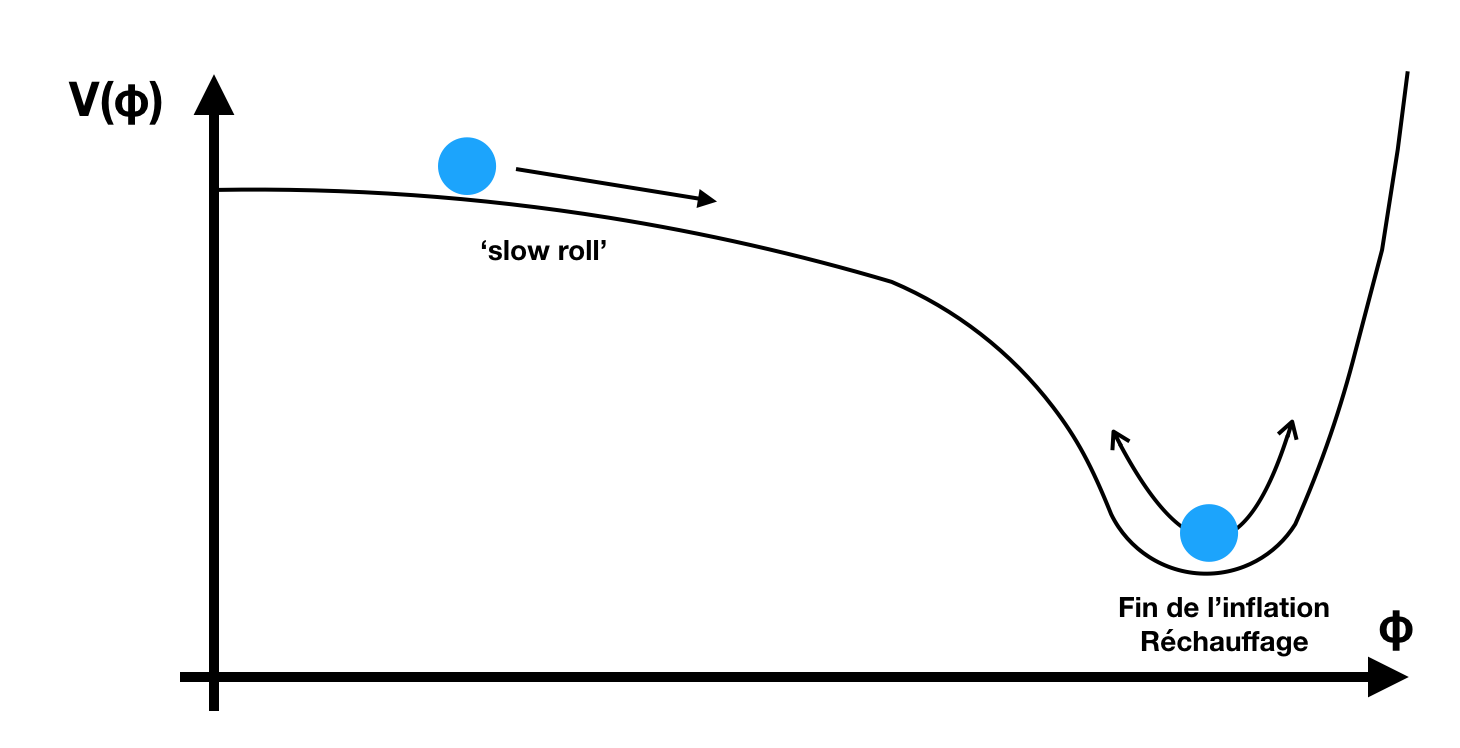
\includegraphics[height=25cm]{figs/slowroll.png}
	\caption[Un exemple de potentiel possible pour l'inflaton. ]{Un exemple de potentiel possible pour l'inflaton. On distingue 2 phases. D'abord une phase où le potentiel est très plat et durant laquelle l'inflaton 'roule' doucement pour produire une phase d'expansion exponentielle. Dans un second temps, l'inflaton se trouve piégé dans un puit de potentiel, stoppant l'inflation et durant laquelle l'énergie libérée est réinjectée dans les autres composantes du cosmos (le réchauffage).}
	\label{f:slowroll}
\end{figure}

\newthought{Le potentiel de l'inflaton} doit donc être choisi avec précaution pour que l'inflation associée ait les bonnes propriétés. Par exemple, on veut un comportement similaire à celui de l'énergie du vide, pour laquelle nous avions $p=-\rho$~: au vu des expressions obtenues pour $\rho_\phi$ et $p_\phi$ cela est possible si le champ scalaire varie lentement
\begin{equation}
\rho_\phi\sim -p_\phi \leftrightarrow \dot \phi \sim 0.
\end{equation}
Or une variation lente de $\phi$ n'est possible que si le potentiel $V(\phi)$ est suffisamment 'plat' pour que l'inflaton puisse 'rouler' lentement le long de sa pente. On parle de condition de \textit{slow-roll}\index{inflation!slow-roll}, condition qui doit être satisfaire par $V(\phi)$ pour que l'inflation ait lieu. Mathématiquement, on souhaite donc que le potentiel ait une pente et une courbure aussi faible que possible:
\begin{eqnarray}
|V'(\phi)|\equiv|\frac{d V}{d\phi}| &\ll& 1\\
|V''\phi)|\equiv|\frac{d ^2 V}{d\phi^2}| &\ll& 1.
\end{eqnarray}
De plus, l'inflation doit s'arrêter à un moment et d'après l'équation \ref{e:hubbleinf} on constate que cela peut s'obtenir si le champ reste bloqué au minimum du potentiel : on a alors $V(\phi)\sim 0$ et $\dot \phi \sim 0$. Il faut donc que le champ 'roule' lentement vers le minimum du potentiel. 

Pour finir, l'inflation va drastiquement diminuer les densités d'énergie de toutes les composantes autres que le l'inflaton (matière, rayonnement, etc...) et pourtant l'une des conditions d'un modèle d'inflation satisfaisant est qu'il puisse se raccrocher à un modèle de Big-Bang chaud standard une fois la phase d'expansion exponentielle terminée. Pour ce faire, l'inflation doit s'accompagner d'une phase de \textit{réchauffage}\index{inflation!réchauffage}, durant laquelle, l'énergie de l'inflaton se déverse dans les réservoirs des autres composantes : on peut montrer par exemple que ce processus de réchauffage opère lorsque l'inflaton oscille au fond du puit créé par le minimum de $V(\phi)$.


En résumé, il existe tout un ensemble de potentiels pouvant satisfaire ces conditions et l'un des objectifs de la cosmologie de l'inflation est précisément de déterminer quel $V(\phi)$ est effectivement à l'oeuvre si l'inflation a bien eu lieu.



\section{Quelques contraintes}
Si toutes ces conditions sont satisfaites alors $H=\dot a /a \sim \mathrm{constante}$ et l'expansion est quasi exponentielle. L'ensemble des problèmes mentionnés en début de chapitre sont résolus si le facteur d'échelle augmente d'un facteur $10^{30}$ entre le début et la fin de l'inflation \sidenote{ici $i$ et $f$ désignent respectivement les instants initiaux et finaux}:
\begin{equation}
a_\mathrm{f}\sim 10^{30} a_\mathrm{i}.
\end{equation}
Ceci permet de mettre une contrainte sur le potentiel de l'inflaton. Ayant $H=\dot a/a$, nous avons ainsi \sidenote{en utilisant l'équation de conservation de la densité d'énergie en approximation de 'slow-roll'}:
\begin{equation}
\log \frac{a_f}{a_i}=\int_{t_i}^{t_f} H dt \sim \int_{\phi_i}^{\phi_f}\frac{V}{V'}d \phi.
\end{equation}
et au vu de l'expansion souhaitée ($10^{30}$ ici), la pente relative du potentiel est ainsi contrainte.

Par ailleurs, le modèle d'inflation permet de prédire l'amplitude du spectre de fluctuation de densité, toujours en fonction de la forme du potentiel :
\begin{equation}
\delta_k\sim \left(\frac{V^{3/2}}{|V'|}\right)_{k=aH/c}.
\end{equation}
L'amplitude du mode $k$ est ainsi déterminée par la valeur du potentiel au moment où le mode sort de l'horizon durant l'inflation. L'observation des fluctuations de densité, par exemple dans le CMB, permet de contraindre davantage la forme du potentiel de l'inflaton, ainsi que les valeurs typiques d'énergie associée. Par exemple l'amplitude mesurée des fluctuations du CMB indique que $V^{1/4}\sim 10^{16}$ GeV\index{inflation!énergie}, bien au delà des énergies accessibles par les accélérateurs terrestre : cela confirme davantage que l'étude de l'époque de l'inflation permettrait d'accéder à des régimes de physiques bien plus extrêmes que ceux auxquels nous sommes habitués. \sidenote{pour référence les énergies actuellement obtenues au LHC (CERN) sont de l'ordre de $10^4$ GeV et celles mesurées pour les rayons cosmiques les plus énergétiques sont de l'ordre de $10^11$ GeV.} En terme d'époques, cela nous place entre $10^{-36}$ et $10^{-30}$ secondes après le Big-Bang. 

Grâce à cette relation le modèle d'inflation permet de prédire la pente du spectre primordial\index{spectre primordial}\index{inflation!spectre}, invariant d'échelle, de fluctuations de densité :
\begin{equation}
\delta^2_k\sim k^n
\end{equation}
et on peut montrer que 
\begin{equation}
n\sim 1-\epsilon -\eta
\end{equation}
où $\epsilon\sim (\frac{V'}{V})^2$ et $\eta \sim \frac{V''}{V}$ qui par condition de 'slow-roll' sont de petites valeurs. A nouveau, la mesure de ce spectre dans par exemple les fluctuations du CMB permet de contraindre la forme du potentiel de l'inflaton. On note que la pente du spectre, $n$ est proche de 1 mais différente de l'unité et les mesures du satellite Planck indique par exemple une valeur de$n\sim 0.97$, ce qui est cohérent avec les prédictions du modèle d'inflation.

Enfin, l'inflation va aussi générer un train d'ondes gravitationnelles primordiales\index{ondes gravitationnelles!inflation} : ces ondes ne vont pas affecter la croissance des structures mais peuvent se manifester dans les propriétés du fond diffus cosmologique \sidenote{notamment dans les cartes mesurant la polarisation du rayonnement}.
On peut montrer que le rapport d'amplitude entre les fluctuations de densité et ces ondes gravitationnelles est donné par
\begin{equation}
R\sim \epsilon.
\end{equation}
Comme vu précédemment $\epsilon$ est faible devant l'unité, impliquant que ces ondes gravitationnelles sont intrinsèquement difficiles à mesurer, sans même considérer les difficultés pratiques qu'implique leur détection. La mesure de ces ondes constituent néanmoins un grand défi de la cosmologie future et dans la validation du modèle d'inflation : ce modèle, quel que soit la forme du potentiel d'inflaton choisi, prédit une relation univoque entre l'amplitude de ces ondes et la forme du spectre de fluctuation:
\begin{equation}
R=-2\pi n_G
\end{equation}
où $A_k\sim k^{n_G}$ est le spectre des ondes gravitationnelles de l'inflation. La confirmation (ou l'invalidation) de cette relation serait une étape essentielle pour établir l'inflation comme étant la bonne solution à tous les problèmes mentionnés en introduction et comme étant la bonne description des processus à l'oeuvre dans l'Univers à ses tous débuts. C'est l'un des grands défis de la cosmologie du futur.